\section{Classification Results}
\setlength{\parindent}{10ex}
%Maybe reword this opening chapter???
In order to iterate on the results displayed in the previous chapter this problem was converted from a continuous prediction to a classification problem.
Conversion was executed by mapping the bathymetry values into discrete classes.
This conversion proved to be trivial because of the ordered nature of bathymetry.
Classification models are simpler and easier to fit than regression models.
Ideally, the decision surfaces will benefit from the conversion and yield better results.
Classification models predict labels and not continuous values.
This makes it difficult to compare directly to the error reported in existing physics models.
A set of metrics including: precision, recall, f1 score, and balanced accuracy were used to analyze the viability of the models.

\par
The ordinal classes were binned on a interval of 150 meters.
This was done to easily compare accuracy to model in \cite{jena2012prediction}.
Validation was preformed using a 10 fold cross validation using balanced accuracy as the scoring function.

\begin{table}[htb]
    \centering
    \begin{tabular}{|c c c|}
        \hline
		\textbf{Model} & \textbf{Average F1 Score} & \textbf{Mean Balanced Accuracy} \\
		\hline
		Random Forest & 0.81 & 0.82 \\
        Bagging & 0.80 & 0.79 \\
        Decision Tree & 0.44 & 0.47 \\
        \hline
    \end{tabular}
    \label{table:CLASSIFICATION_RESULTS}
    \caption{Classification Results}
\end{table}

\subsection{Classification Results Discussion}
The Random Forest model performed excellently with a balanced accuracy of 82\%.
Breaking down the results by class, the classifier predicted some classes with greater precision than others.
This is indicative that the decision boundary responded to certain trends in the data.

\par
The Bagging classifier performed on par with the Random Forest Classifier with a balanced accuracy of 79\%.
As seen with \ac{RFC}, bagging performed better at predicting some classes than others.
Again indicating that the decision boundary responded to certain trends in the data.

\par
The Decision Tree classifier performed significantly worse than the other models.
The 47\% balanced accuracy is not usable for predictions.
Potentially, parameter tuning, and maybe feature selection could improve this model.

\par
Classification shows that labeling bathymetry can improve the performance of the models.
However, what is more interesting to analyze is the behavior of the models.
The data used in training comes from aggregated external datasets and a predicted bathymetry dataset.
The predictions of these models is being compared to predicted bathymetry which represents the accuracy with relation to predicted values.
Meaning that the accuracy in these models is not indicative of truly predicting global bathymetry.
It does show that a \ac{ML} model can be fit to data and used to predict bathymetry, and if actual measured bathymetry and ocean features were used in training the results would be comparable.
Furthermore, parameter tuning, model selection, and dynamic feature selection could be used the increase the accuracy beyond current results.

\begin{figure}[hb]
    \centering
    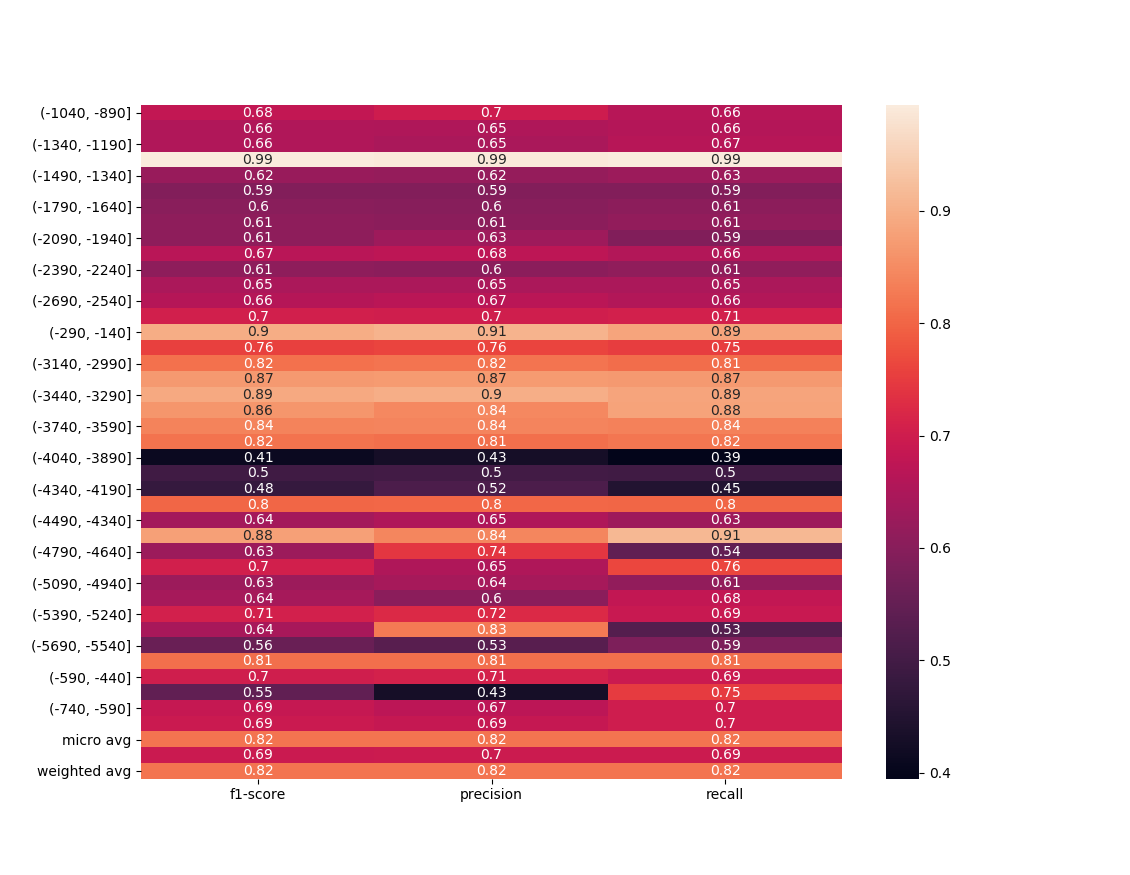
\includegraphics[width=\textwidth]{rfc_class_report.png}
    \caption{Figure displaying the heat map classification report of the Random Forest Classifier}
    \label{fig:rfc_report}
\end{figure}

\par
Figure \ref{fig:rfc_report} displays the classification report for the Random Forest Classifier along a reduced selection of classes.
Precision and recall are excellent measurements to show the performance of a classifier.
What is interesting in figure \ref{fig:rfc_report} is that the precision and recall differs drastically between classes.
This suggests that a classifier will perform different based on the depth.
It also suggests that other localized factors could impact the decision boundaries as the depths are tied to a physical location.
